\documentclass[
    pdftex,
    12pt,
    parskip=half,
    a4paper
]{scrartcl}
\author{Crawford, Sam}
\title{Einführung in Kryptographie und IT-Sicherheit}

\usepackage[utf8]{inputenc}
\usepackage[naustrian]{babel}
\usepackage{graphicx}
\usepackage{listings}
\usepackage{xcolor}
\usepackage{mathtools}
\usepackage{subcaption}

% Define color scheme
\definecolor{codeblue}{rgb}{0.13, 0.13, 0.75}
\definecolor{codegreen}{rgb}{0, 0.5, 0}
\definecolor{codered}{rgb}{0.75, 0.13, 0.13}
\definecolor{codegray}{rgb}{0.5, 0.5, 0.5}
\definecolor{backgray}{rgb}{0.95, 0.95, 0.95}

% Define Python style for listings
\lstdefinestyle{pythonstyle}{
    language=Python,
    basicstyle=\ttfamily,
    keywordstyle=\color{codeblue}\bfseries,
    stringstyle=\color{codered},
    commentstyle=\color{codegreen}\itshape,
    numberstyle=\tiny\color{codegray},
    numbers=left,
    stepnumber=1,
    numbersep=10pt,
    backgroundcolor=\color{backgray},
    showspaces=false,
    showstringspaces=false,
    frame=single,
    tabsize=3,
    breaklines=true,
    breakatwhitespace=true,
}
\lstset{style=pythonstyle}

\usepackage[naustrian]{babel}

\begin{document}
\maketitle

\section{Implementierung der Baker's Map}
Siehe \ref{sec:bakersmap} für eine Baker's Map Erklärung. Die gewählte Programmiersprache ist Python.
Für Bilder wird die Library OpenCV verwendet. Der Programmcode zur Verschlüsselung ist folgender:
\begin{lstlisting}
\end{lstlisting}

\section{Chaos-basierte Bildverschlüsselung und Entschlüsselung}
\subsection{Motivation}
% TODO: 
TODO: Main motivations from his article: less computational effort (than AES) and more security benefits.

Für die Verschlüsselung von Bildern wird eine Methode benötigt, die den Inhalt
versteckt. Bilder bestehen aus einer Struktur von Pixeln, d.h. es ist relevant welche Pixel neben welchen
Pixeln liegen. Weiters weisen Bilder eine hohe Redundanz auf. Traditionelle Verschlüsselungsmethoden beachten
diese Aspekte bei Bildern nicht wirklich und somit ist eine andere Verschlüsselungsmethode erforderlich.
Chaos-basierte Verschlüsselung ist deterministisch, hat eine hohe Ergodizidät, d.h. es werden praktisch alle
möglichen Zustände des Systems über einen längeren Zeitraum angenommen, und weist Pseudo-Zufälligkeit auf. Außerdem
sind sie sehr sensibel zu den Ausgangsbedingungen, d.h. kleine Veränderungen der Ausgangsbedingungen führen zu
sehr anderen Ergebnissen. Das bedeutet, dass aufgrund der Komplexität solcher Systeme es schwer ist,
das Verhalten vorherzusehen.
Somit sind chaos-basierte Verschlüsselungen von Vorteil für die Verschlüsselung von Bildern.
\cite{zhang2023}

\subsection{Funktionsweise} % TODO: make it fit with below subsections
Die chaos-basierte Verschlüsselung nutzt eine chaotische Abbildung wie die Baker Map oder Cat Map. Beide bilden
einen 2-dimensionalen Einheitsquadrat auf sich selber ab. Der Grund warum diese Abbildungen gewählt werden ist, da
sie relativ simpel sind und somit schnell verschlüsselt/enschlüsselt werden kann. 
Eine solche Abbildung wird dann im nächsten Schritt generalisiert, indem Parameter zur Abbildung hinzugefügt werden.
Danach wird sie diskretisiert, denn ein Bild besteht aus diskreten Pixeln. Das bedeutet, dass die Abbildung so
modifiziert wird, sodass sie nicht mehr ein Einheitsquadrat auf sich selbst abbilden, sondern ein 2-dimensionales quadratisches
Bild bestehend aus Pixeln auf sich selber abbildet. So eine Abbildung bestimmt also eine Bijektion zwischen den einzelnen Pixeln
quadratischer Bilder, sodass eine Permutation der Pixel berechnet werden kann. Anschließend wird die Abbildung auf 3 Dimensionen erweitert,
sodass einzelne Pixel Werte modifiziert werden. Schlussendlich wird dann eine Diffusion noch angewendet als Komposition zur bestehenden
Abbildung.
\cite{IEEEMap}

Zur Entschlüsselung wird dann die inverse Baker Map verwendet, sodass man das Ursprungsbild wieder erhaltet nach gleich vielen Iterationen.

\subsubsection{Cat Map}
Die generalisierte Cat Map Transformation $\Gamma$ ist folgendermaßen definiert:
$$
	\Gamma:
	\begin{bmatrix} x \\ y \end{bmatrix} \rightarrow
	\begin{bmatrix} 1 & p \\ q & pq + 1 \end{bmatrix}
	\begin{bmatrix} x \\ y \end{bmatrix} \text{ mod } n
$$
Wobei $X = \begin{bmatrix} x & y \end{bmatrix}^T$ ein Pixel von einem $n \times n$ Bild mit $1 \leq x \land y \leq n$.
Dabei sind $p \geq 1$ und $q \geq 1$ Teil des Schlüssels mit $t$, wobei $t$ die Anzahl der Iterationen entspricht. \cite{chaos}

\subsubsection{Baker's Map}\label{sec:bakersmap}
Die Baker's Map ist eine chaotische Abbildung, die das Bild $N \times N$ vertikal teilt, horizontal streckt und die Teile aufeinander stapelt, ähnlich
wie ein Bäcker mit Teig umgeht, daher der Name. Der Schlüssel hier ist durch die Anzahl an Rechtecke und die Position der Teilungen gegeben. \cite{chaos}

Die Abbildung funktioniert folgendermaßen: Man definiere zuerst $n_1, n_2, \dots , n_k$, wobei $k$ die Anzahl der aufgeteilten Teile entspricht.
Dabei muss $\forall i \in \{1, 2, \dots, k\} : n_i | N$ und $\sum_{i = 1}^{k} n_i = N$ gelten. Sei weiter $N_i \coloneq \sum_{j = 1}^{i} n_j$ und $q_i \coloneq N/n_i$.
Betrachte nun ein Pixel ($r$, $s$) mit $N_{i - 1} \leq r < N_i$ und $0 \leq s < N$. Dieses Pixel wird abgebildet auf:
$$B(r, s) =  (q_i(r - N_i) + (s \text{ mod } q_i), \frac{s - (s \text{ mod } q_i)}{q_i + N_i})$$
Dieser Algorithmus ist verantwortlich für eine Permutation der Pixel. Um die Grauwerte der Pixel auch zu verändern, kann ein Substitutionsschritt
eingeführt werden, der den Grauwert $g_{rs}$ eines Pixels beim Abbilden ändert auf $h(r, s, g_{rs})$, wobei $h$ folgende Funktion ist:
$$h(r, s, g_{rs}) = (g_{rs} + r \cdot s) \text{ mod } L$$
Dabei ist $L$ die Anzahl an Grauwerten.
\cite{chaos}

\section{Verschlüsselung mit AES}
Die gewählte Programmiersprache ist Python. Für die Verschlüsselung wurde PyCryptdome verwendet.
Bilder werden mit OpenCV behandelt.
Dies ist der Programmcode, für die Verschlüsselungsfunktion:
\begin{lstlisting}
import cv2
from Crypto.Cipher import AES

def encrypt_image(key, image):
    width, height = image.shape
    flat_original = image.flatten()
    flat_encrypted = flat_original.copy()
    ivs = []

    for i in range(0, len(flat_original), 16):
        cipher = AES.new(key, AES.MODE_CBC)
        ivs.append(cipher.iv)
        pixels = flat_original[i : i + 16]

        encrypted_bytes = cipher.encrypt(b"".join(pixels))
        for j in range(16):
            flat_encrypted[i + j] = encrypted_bytes[j]

    encrypted_image = flat_encrypted.reshape((width, height))
    return ivs, encrypted_image
\end{lstlisting}
Die Funktion \lstinline{encrypt_image()} besitzt zwei Parameter: einen Schlüssel und das Bild,
das man verschlüsseln möchte. Als Erstes werden die Seitenlängen des Bildes gespeichert. Dann wird das 2D-Bild-Array
mit \lstinline{.flatten()} zu einem 1D-Array umgewandelt für leichtere Handhabung. Außerdem wird ein weiteres 1D-Array
gleicher Länge angelegt, wo die verschlüsselten Pixel später platziert werden.

In den Zeilen 10 bis 17 ist dann der Hauptalgorithmus. Für jede 16 Elemente des 1D-Arrays wird ein neuer Cipher erstellt,
dessen Initialisierungsvektor \lstinline{iv} in die \lstinline{ivs} Liste gespeichert wird. Anschließend werden die 16 Elemente,
also 16 Bytes, zu einem 16-Byte-Block (128-Bit) zusammengeführt und mithilfe dem Cipher verschlüsselt.
Dann wird an jene Stellen, von denen die ursprünglichen Bytes kommen, die verschlüsselten
16 Bytes als verschlüsselte Pixel in das neue 1D-Array gesetzt. Nachdem der äußerste for-loop terminiert, wird das neu befüllte 1D-Array in ein
Bild umgewandelt, welches dann mit \lstinline{ivs} als 2-Tupel zurückgegeben wird.

Zum Entschlüsseln benötigt man denselben Schlüssel und die Initialisierungsvektoren. Die Funktion dazu ist diese hier:
\begin{lstlisting}
def decrypt_image(ivs, key, image):
    width, height = image.shape
    flat_encrypted = image.flatten()
    flat_decrypted = flat_encrypted.copy()

    for i in range(0, len(flat_encrypted), 16):
        cipher = AES.new(key, AES.MODE_CBC, iv=ivs[i // 16])
        pixels = flat_encrypted[i : i + 16]

        decrypted_bytes = cipher.decrypt(b"".join(pixels))
        for j in range(16):
            flat_decrypted[i + j] = decrypted_bytes[j]

    return flat_decrypted.reshape((width, height))
\end{lstlisting}
Der Algorithmus ist analog zu \lstinline{encrypt_image()}. Die 2D-Arrays werden in 1D-Arrays umgewandelt. Dann wird für alle
16 Bytes diese 16 Bytes mithilfe des Schlüssels und dem jeweiligen Initialisierungsvektor entschlüsselt. Anschließend werden diese entschlüsselten Bytes
bei dem neuen 1D-Array entsprechend ihrer ursprünglichen Positionen gesetzt. Als Letztes wird dann dieses entschlüsselte 1D-Array
in ein 2D-Bild-Array zurückgewandelt und man hat somit das verschlüsselte Bild entschlüsselt.

Somit könnte das Hauptprogramm folgendermaßen vorgehen:
\begin{lstlisting}
import sys

def main():
    image = cv2.imread(sys.argv[1])
    image = cv2.cvtColor(image, cv2.COLOR_BGR2GRAY)
    show_image_with_entropy(image)

    cipher_key = b"my 16 byte key!!"
    ivs, encrypted_image = encrypt_image(cipher_key, image)
    show_image_with_entropy(encrypted_image)

    decrypted_image = decrypt_image(ivs, cipher_key, encrypted_image)
    show_image_with_entropy(decrypted_image)
\end{lstlisting}
Der Name des Bildes wird als Kommando-Zeilen-Argument übergeben. Es wird dann eingelesen und in Grayscale konvertiert.
Dann wird mit dem key \lstinline{cipher_key} das Bild verschlüsselt mithilfe \lstinline{encrypt_image()} und danach
mit demselben Schlüssel und den erhaltenen Initialisierungsvektoren mit der Funktion \lstinline{decrypt_image()} entschlüsselt.

\subsection{Verschlüsseln von 10 Bildern}
Für konkrete Beispiele mit den jeweiligen Entropien, siehe Abbildungen \ref{fig:cat} bis \ref{fig:sky}.

\subsection{Zeitbedarf der Verschlüsselung}
Was den Zeitbedarf der Verschlüsselung betrifft: Die Ausführung des Programms dauert im Durchschnitt
$613.79$ Millisekunden.
Die Tabelle \ref{tab:speed3} gibt die konkreten Werte pro Bild an, wobei die Nummerierungen der Bilder
der Ordnung der Bilder entsprechen.
\begin{table}
	\begin{center}
		\begin{tabular}{ |c|c|c| } 
		\hline
		Bild & Zeit (in Millisekunden) \\
		\hline
		1 & 623.05 \\
		2 & 598.61 \\
		3 & 617.41\\
		4 & 598.53\\
		5 & 603.35\\
		6 & 605.35\\
		7 & 620.01\\
		8 & 608.46\\
		9 & 636.87\\
		10 & 626.23\\
		\hline
		\end{tabular}
	\end{center}
	\caption{Die individuellen Zeiten um ein Bild zu verschlüsseln}
	\label{tab:speed3}
\end{table}

\begin{figure}
	\centering

	\begin{subfigure}{0.35\textwidth}
		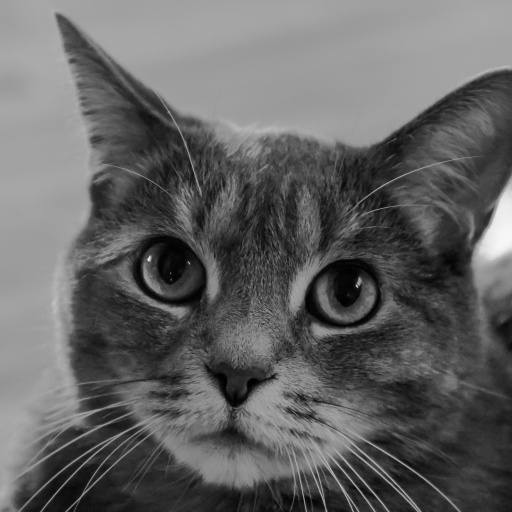
\includegraphics[width=\textwidth]{../1/3/gray_7.055047578254635_cat.jpg}
		\caption{Entropie: 7.055047578254635}
	\end{subfigure}
	\hfill
	\begin{subfigure}{0.35\textwidth}
		
\includegraphics[width=\textwidth]{../1/3/encrypted_7.9993452182261775_cat.jpg}
		\caption{Entropie: 7.999345218226177}
	\end{subfigure}

	\caption{Bild vor (a) und nach (b) Verschlüsselung}
	\label{fig:cat}
\end{figure}

\begin{figure}
	\centering

	\begin{subfigure}{0.35\textwidth}
		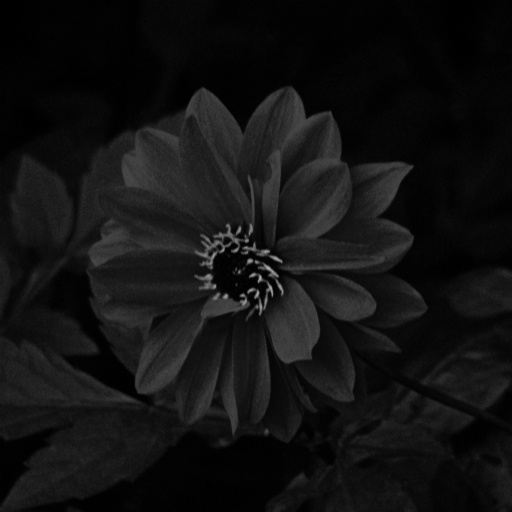
\includegraphics[width=\textwidth]{../1/3/gray_5.489817933250877_flower.jpg}
		\caption{Entropie: 5.489817933250877}
	\end{subfigure}
	\hfill
	\begin{subfigure}{0.35\textwidth}
		
\includegraphics[width=\textwidth]{../1/3/encrypted_7.999288647342163_flower.jpg}
		\caption{Entropie: 7.999288647342163}
	\end{subfigure}

	\caption{Bild vor (a) und nach (b) Verschlüsselung}
	\label{fig:flower}
\end{figure}

\begin{figure}
	\centering

	\begin{subfigure}{0.35\textwidth}
		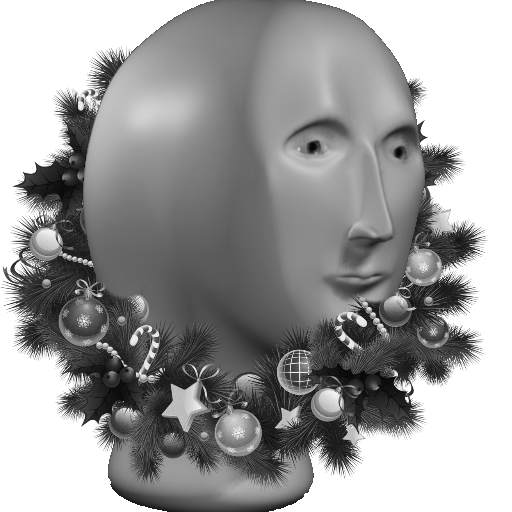
\includegraphics[width=\textwidth]{../1/3/gray_6.176106420718194_meme_man.png}
		\caption{Entropie: 6.176106420718194}
	\end{subfigure}
	\hfill
	\begin{subfigure}{0.35\textwidth}
		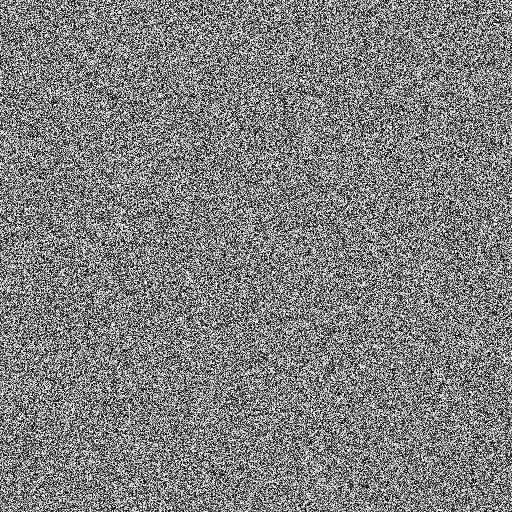
\includegraphics[width=\textwidth]{../1/3/encrypted_7.999330312791573_meme_man.png}
		\caption{Entropie: 7.999330312791573}
	\end{subfigure}

	\caption{Bild vor (a) und nach (b) Verschlüsselung}
	\label{fig:meme_man}
\end{figure}

\begin{figure}
	\centering

	\begin{subfigure}{0.35\textwidth}
		
\includegraphics[width=\textwidth]{../1/3/gray_1.968975268089162_spheal.png}
		\caption{Entropie: 1.968975268089162}
	\end{subfigure}
	\hfill
	\begin{subfigure}{0.35\textwidth}
		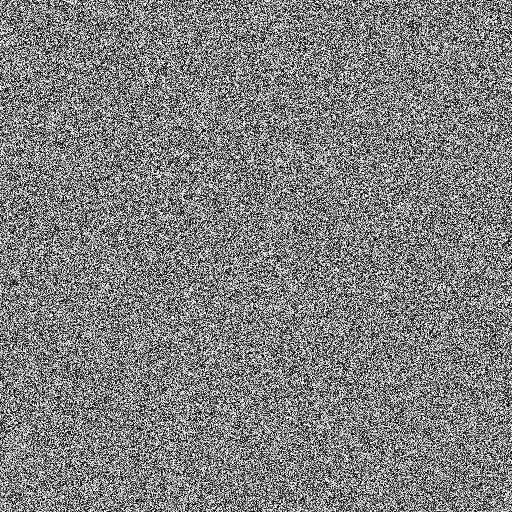
\includegraphics[width=\textwidth]{../1/3/encrypted_7.999276890528033_spheal.png}
		\caption{Entropie: 7.999276890528033}
	\end{subfigure}

	\caption{Bild vor (a) und nach (b) Verschlüsselung}
	\label{fig:spheal}
\end{figure}

\begin{figure}
	\centering

	\begin{subfigure}{0.35\textwidth}
		
\includegraphics[width=\textwidth]{../1/3/gray_4.1555418953746175_frog.jpg}
		\caption{Entropie: 4.155541895374617}
	\end{subfigure}
	\hfill
	\begin{subfigure}{0.35\textwidth}
		
\includegraphics[width=\textwidth]{../1/3/encrypted_7.999333134306007_frog.jpg}
		\caption{Entropie: 7.999333134306007}
	\end{subfigure}

	\caption{Bild vor (a) und nach (b) Verschlüsselung}
	\label{fig:frog}
\end{figure}

\begin{figure}
	\centering

	\begin{subfigure}{0.35\textwidth}
		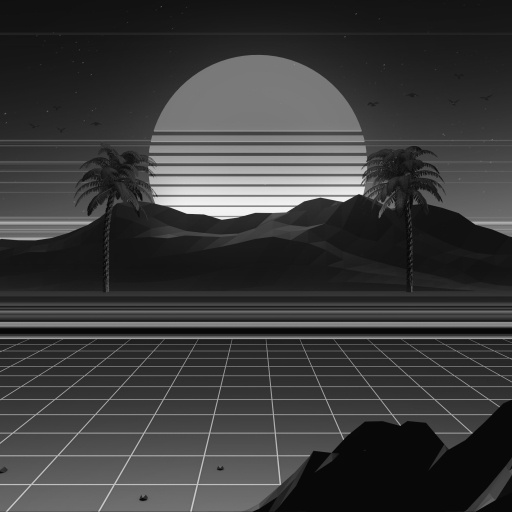
\includegraphics[width=\textwidth]{../1/3/gray_6.761302835772753_synthwave.jpg}
		\caption{Entropie: 6.761302835772753}
	\end{subfigure}
	\hfill
	\begin{subfigure}{0.35\textwidth}
		
\includegraphics[width=\textwidth]{../1/3/encrypted_7.999245942902867_synthwave.jpg}
		\caption{Entropie: 7.999245942902867}
	\end{subfigure}

	\caption{Bild vor (a) und nach (b) Verschlüsselung}
	\label{fig:synthwave}
\end{figure}

\begin{figure}
	\centering

	\begin{subfigure}{0.35\textwidth}
		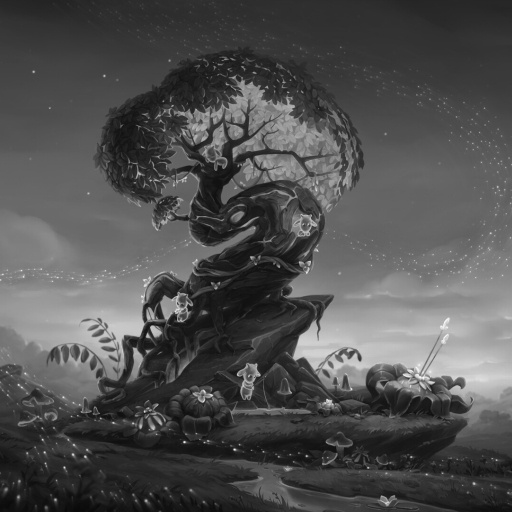
\includegraphics[width=\textwidth]{../1/3/gray_7.2193250947721515_fantasy_tree.jpg}
		\caption{Entropie: 7.219325094772151}
	\end{subfigure}
	\hfill
	\begin{subfigure}{0.35\textwidth}
		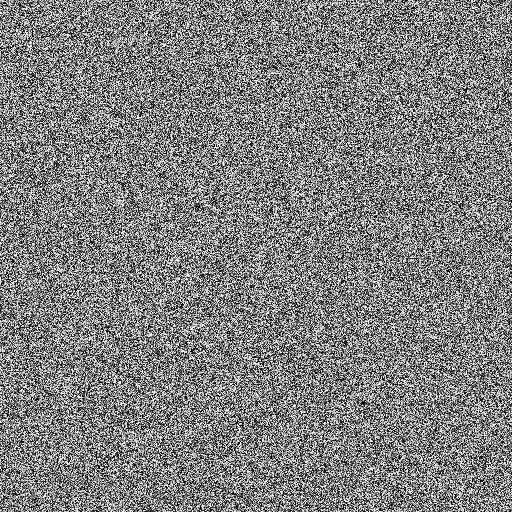
\includegraphics[width=\textwidth]{../1/3/encrypted_7.999253958586079_fantasy_tree.jpg}
		\caption{Entropie: 7.999253958586079}
	\end{subfigure}

	\caption{Bild vor (a) und nach (b) Verschlüsselung}
	\label{fig:fantasy}
\end{figure}

\begin{figure}
	\centering

	\begin{subfigure}{0.35\textwidth}
		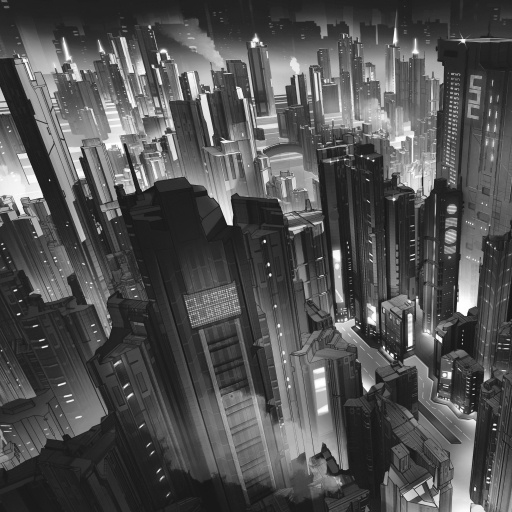
\includegraphics[width=\textwidth]{../1/3/gray_7.228465731556658_city.jpg}
		\caption{Entropie: 7.228465731556658}
	\end{subfigure}
	\hfill
	\begin{subfigure}{0.35\textwidth}
		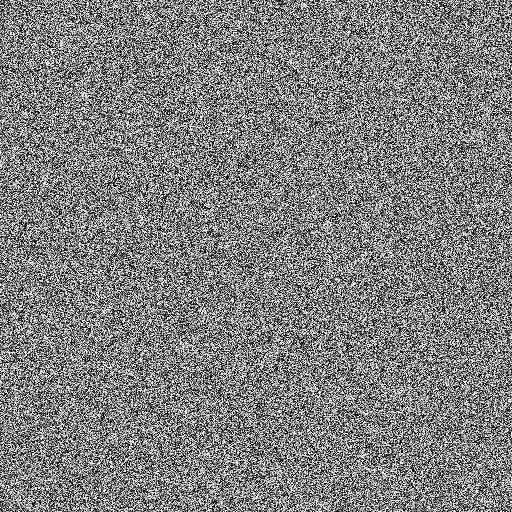
\includegraphics[width=\textwidth]{../1/3/encrypted_7.999299251892032_city.jpg}
		\caption{Entropie: 7.999299251892032}
	\end{subfigure}

	\caption{Bild vor (a) und nach (b) Verschlüsselung}
	\label{fig:city}
\end{figure}

\begin{figure}
	\centering

	\begin{subfigure}{0.35\textwidth}
		
\includegraphics[width=\textwidth]{../1/3/gray_6.920844020928125_pikachu.jpg}
		\caption{Entropie: 6.920844020928125}
	\end{subfigure}
	\hfill
	\begin{subfigure}{0.35\textwidth}
		
\includegraphics[width=\textwidth]{../1/3/encrypted_7.999437945674354_pikachu.jpg}
		\caption{Entropie: 7.999437945674354}
	\end{subfigure}

	\caption{Bild vor (a) und nach (b) Verschlüsselung}
	\label{fig:pika}
\end{figure}

\begin{figure}
	\centering

	\begin{subfigure}{0.35\textwidth}
		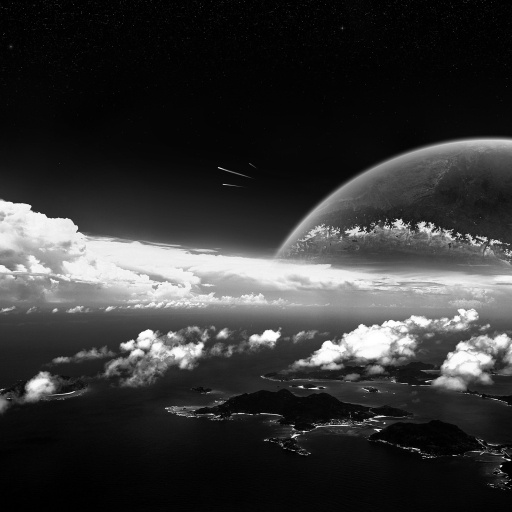
\includegraphics[width=\textwidth]{../1/3/gray_6.636128377207226_planet_sky.jpg}
		\caption{Entropie: 6.636128377207226}
	\end{subfigure}
	\hfill
	\begin{subfigure}{0.35\textwidth}
		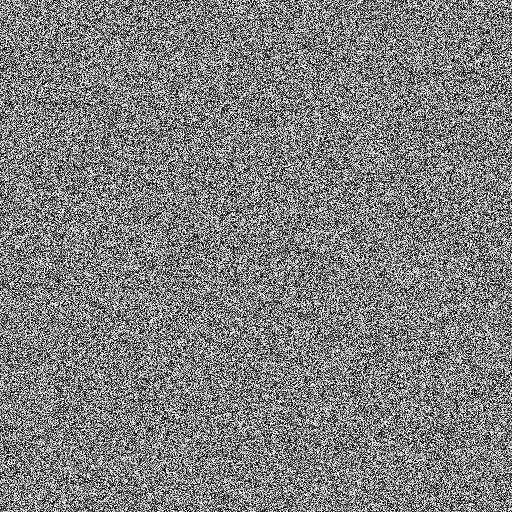
\includegraphics[width=\textwidth]{../1/3/encrypted_7.999257183679586_planet_sky.jpg}
		\caption{Entropie: 7.999257183679586}
	\end{subfigure}

	\caption{Bild vor (a) und nach (b) Verschlüsselung}
	\label{fig:sky}
\end{figure}


\section{Artikel lesen/erklären}
Die Autoren dieses Artikels, siehe \cite{chaos}, sind der Meinung, dass Chaos-basierte Bildverschlüsselung
unseriös/ungeeignet ist. Die Punkte, die sie kritisieren, sind folgende:

Eines der Motivationen von Chaos-basierter Bildverschlüsselung ist der behauptete geringere Rechenaufwand.
Ein Vorteil von solcher Verschlüsselung sei, dass es weniger Rechenarbeit als andere schon bestehende
Verfahren wie z.B. AES, das in \cite{chaos} als Vergleich hergenommen wurde, benötigt. In ihren Experimenten
zeigen sie aber sogar das Gegenteil: Chaos-basierte Verschlüsselungsmethoden sind nicht effizienter und oft
nicht ansatzweise so schnell wie traditionelle Methoden aus hochoptimierten kryptografischen Libraries. Die Autoren
schätzen auch ein, dass dies sich nicht ändern wird.

Eine weitere Motivation von Chaos-basierter Bildverschlüsselung ist bezogen auf die daraus resultierende Sicherheit.
Laut \cite{chaos} wird in vielen Publikationen behauptet, dass Bilder eine hohe Redundanz aufweisen, d.h. dass Information vorhersehbar oder
stark wiederholt wird und dass das nicht bei konventionellen Methoden beachtet wird. Dem widersprechen aber die Autoren von \cite{chaos},
solange man beispielsweise bei AES Modi verwendet, die dies beachten, da die Verschlüsselung unabhängig vom Originalmaterial ist. (Sie nennen
CBC, OFB und Counter Mode)

Vor allem aber kritisieren sie die Publikationen, die ein neues Verfahren vorstellen, das sie
nur experimentell ``beweisen'', indem z.B. Entropien gemessen werden
oder Grayscale-Histogramme betrachtet werden. Ein weiterer Punkt ist meist die kleine Menge an Bildern, an welchen diese Experimente durchgeführt werden.

Die Autoren aus \cite{chaos} kritisieren diese Tests vor allem, da sie so verwendet werden, als wären sie ausreichend für eine hohe Sicherheit, obwohl
sie eigentlich eine Grundbedingung für eine hohe Sicherheit sind. Es gibt einige konkrete Fälle, bei welchen ein Verfahren nach dem Durchlaufen
von solcher Tests als sicher eingestuft wurde, nur um ein Jahr später durch bereits bekannte Verfahren geknackt zu werden.

Somit kritisieren die Autoren von \cite{chaos} nicht nur die Verschlüsselungsmethoden selber, sondern auch die Arbeitsweise von denjenigen, die
diese Verfahren vorstellen.

\section{Fehlerkorrektur mit Hammingcodes}

\subsection{Funktionsweise} \label{sec:hammingfunc}
Ein Hammingcode kann einerseits Fehler erkennen und andererseits auch einen Fehler korrigieren.
Dies funktioniert folgendermaßen: Einer binären Nachricht der Länge $2^m - m - 1$ wird $m$ redundante Bits
hinzugefügt, sodass das der Code eine Länge von $2^m - 1$ hat. Die redundanten Bits sind an den $2^n$-ten Stellen positioniert, wobei
die linkeste Stelle mit dem MSB die erste Stelle ist.
Sei $p_i$ das redundante Bit an der Stelle $2^{i - 1}$. Verwendet werden diese Bits als Paritätsbits, d.h. entweder Even oder Odd Parity.
Angenommen es wird Even Parity verwendet. Dann wird der Wert eines Paritätsbit bestimmt, indem die Anzahl an 1en aller dazugehörigen Bits
gezählt wird. Wenn diese ungerade ist, ist das Paritätsbit $1$, sonst $0$. Zu einem Paritätsbit $p_i$ gehören alle Bits an den Stellen
(beginnend von 1), wo die Binärdarstellung der Stelle eine $1$ an der $i$-ten Stelle von rechts aufweist. Beispielsweise gehört zu dem Paritätsbit $p_1$
jedes Bit an einer ungeraden Stelle, da ungerade Zahlen immer eine 1 an der 1. Stelle von rechts aufweisen. Wenn alle zugehörigen Bits mit dem
Paritätsbit eine gerade Anzahl an 1en haben, dann ist die Even Parity erfüllt. \cite{hamming}

Wenn ein solcher Hammingcode erstellt wurde, kann dieser verschickt werden. Dabei kann es zu Fehlern kommen, also es kommt zu ungewollten
Bit-Flips. Anhand der Paritätsbits kann man nun feststellen, ob es zu so einem Fehler gekommen ist und bei 1-Bit Fehlern sogar ausbessern. \cite{hamming}

Der Empfänger, der diesen möglicherweise fehlerhaften Code erhaltet, muss erstmal für jedes Paritätsbit überprüfen, ob die Even Parity gilt.
Wenn nicht, dann hat der Code einen Fehler. \cite{hamming}

Für die Fehlerkorrektur von einem Bit wird folgendes durchgeführt: Für jedes Paritätsbit wird die Parity berechnet. Wenn sie erfüllt ist, dann
wird in eine neu zu konstruierende Zahl eine 0 hinzugefügt, sonst eine 1. Dies wird von rechts nach links durchgeführt. Die daraus resultierende
Binärzahl ist die Stelle, an der der Fehler geschehen ist, somit muss man nur dieses Bit flippen, um den Fehler zu beheben. \cite{hamming}

\subsection{Beispiel}
Um dies an einem konkreten Beispiel zu demonstrieren: Angenommen man möchte die Bits 1101 übertragen. Dann bräuchte man drei redundante Paritätsbits,
sodass der Code eine Länge von $2^3 - 1$ hat. (mit 3 redundanten Bits) Diese Paritätsbits $p_i$ müssen an den $2^{i - 1}$-ten Stellen platziert werden, also
$p_1 p_2 1 p_3 101$. Dann müssen die Werte von den Paritätsbits gemäß der Beschreibung in Sektion \ref{sec:hammingfunc} gewählt werden.
Der resultierende Hammingcode ist 1010101.

Angenommen dieser Code erleidet an einem Fehler: Das Bit an der 6. Stelle von links wird geflipped, sodass der Code nun
1010111 ist. Dann ist für $p_2$ und $p_3$ die Even Parity nicht mehr erfüllt. Damit man die problematische Stelle findet,
wird in $p_3 p_2 p_1$ das $p_i$ durch 0 ersetzt, wenn die Even Parity nicht erfüllt ist, sonst 1. Somit erhaltet man die Zahl $110_2 = 6_{10}$.
Also ist der Fehler an der 6. Stelle geschehen und muss geflipped werden. Man erhaltet also dann den reparierten Code 1010101,
den man nun wieder gewöhnlich dekodieren kann, um 1101 zu erhalten.

Dieser Prozess ist hier umgesetzt als Python Skript. Verwendet wird die Python Implementierung von Dominic Carrano, die auf
Github\footnote{https://github.com/dominiccarrano/hamming} veröffentlicht ist. Binärzahlen werden mithilfe bitarray dargestellt:
\begin{lstlisting}
import hamming
from bitarray import bitarray
import sys

def main():
    msg = bitarray(sys.argv[1])
    print(f"Original Bits: {msg}")
    print()

    encoded_msg = hamming.encode(msg)
    print(f"Encoded Bits: {encoded_msg}")

    decoded_msg = hamming.decode(encoded_msg)
    print(f"Decoded Bits: {decoded_msg}")
    print()

    # simulating corruption
    corrupt_encoded_msg = encoded_msg.copy()
    corrupt_encoded_msg[6] = corrupt_encoded_msg[6] ^ 1
    print(f"Corrupted encoded Bits: {corrupt_encoded_msg}")

    corrupt_decoded_msg = hamming.decode(corrupt_encoded_msg)
    print(f"Decoded Bits: {corrupt_decoded_msg}")
\end{lstlisting}
Es wird zuerst gemäß dem Kommando-Zeilen-Argument ein bitarray erstellt für die Binärzahl. Danach wird sie in einem
Hammingcode umgewandelt und sofort wieder zurückgewandelt, um das Original zu erhalten. Dies simuliert einen fehlerfreien
Transfer. Nun kann es aber zu Fehlern kommen. Daher wird im Skript ein korrupter Hammingcode erstellt, an dessen 6. Stelle
ein Bit geflipped wird. Aber da es ein Hammingcode ist, kann beim Dekodieren dieser Fehler erkannt und korrigiert werden.
Dies ist die Ausgabe des Programms bei der Eingabe 1101:
\begin{lstlisting}
Original Bits: bitarray('1101')

Encoded Bits: bitarray('01010101')
Decoded Bits: bitarray('1101')

Corrupted encoded Bits: bitarray('01010111')
Decoded Bits: bitarray('1101')
\end{lstlisting}
Der Grund, warum der Hammingcode eine Länge von 8 hat, ist, weil der Autor der Hammingcode Software zusätzlich
zum Hammingcode noch ein Paritätsbit für die ganze Sequenz links einfügt. Da die Sequenz 1010101 eine even Parity hat (vier 1en),
wird links noch zusätzlich das Paritätsbit 0 eingefügt.


\bibliography{lit}
\bibliographystyle{alpha}
\end{document}
